\title{Study Guide for Midterm 2}
\author{Dr. Jordan Hanson - Whittier College Dept. of Physics and Astronomy}
\date{\today}
\documentclass[10pt]{article}
\usepackage[margin=1.5cm]{geometry}
\usepackage{outlines}
\usepackage{graphicx}
\usepackage{amsmath}

\begin{document}
\maketitle

\section{Memory Bank}

\begin{itemize}
\item Unit conversions: 1 km = 1000 m, 1 m = 100 cm, 1 hr = 3600 s, 1 year = $\pi \times 10^7$ s, 1 g/cm$^3$ = 1000 kg/m$^3$.
\item $\vec{x} = a \hat{i} + b\hat{j}$ ... Component form of a two-dimensional vector.
\item $|\vec{x}| = \sqrt{a^2+b^2}$ ... Pythagorean theorem for obtaining vector magnitude.
\item $\theta = \tan^{-1}(b/a)$ ... Obtaining the angle between vector and x-axis.
\item $a = |\vec{x}|\cos(\theta)$ ... Obtaining the x-component with trigonometry.
\item $b = |\vec{x}|\sin(\theta)$ ... Obtaining the y-component with trigonometry.
\item $x(t) = x_i + v t$ ... Velocity is the slope of position versus time.
\item $x(t) = \frac{1}{2} a t^2 + v_i t + x_i$ ... With constant acceleration, position is quadratic.  If $a=0$ this becomes the prior function.
\item $v(t) = v_i + a t$ ... With constant acceleration, acceleration is the slope of velocity.
\item $v^2 = v_i^2 + 2 a \Delta x$ ... The kinematic equation without time, assuming constant acceleration.
\item $\vec{F}_{net} = 0$ ... Newton's First Law, an object with no net force stays at constant velocity, or zero velocity.
\item $\vec{F}_{net} = m\vec{a}$ ... Newton's Second Law.
\item $\vec{F}_{AB} = -\vec{F}_{BA}$ ... Newton's Third Law.
\item $\vec{w} = - mg \hat{j}$ ... Weight force.
\item $\vec{N} = +mg\hat{j}$ ... Normal force, when the object is on a flat surface.
\item $N = mg\cos\theta$, $w_x = -mg\sin\theta$, $w_y = -mg\cos\theta$ ... Incline plane forces.
\item $f = \mu N$, $F_D = \frac{1}{2}C\rho A v^2$, $F_D = 6\pi r \eta v$ ... friction, drag in air, drag in viscous fluids.
\item $stress = Y \times strain$, or $F/A = Y (\Delta x / L)$ ... Young's Modulus and elasticity.
\item $s = r \theta$ ... Definition of a \textit{radian}, with arc length $s$ and angle $\theta$.
\item $v = r\omega$, $a = r\alpha$ ... Angular velocity, angular acceleration.
\item $a_C = v^2/r = r\omega^2$ ... Centripetal acceleration.
\item $F_C = m a_C = mv^2/r = mr\omega^2$ ... Centripetal force.
\item $\vec{F}_G = G m_1 m_2/r^2 ~~ \hat{r}$ ... Newton's Law of Gravity.
\item $dW = \vec{F}(\vec{r}) \cdot d\vec{r}$ ... Definition of work.
\item $W = \vec{F} \cdot \Delta \vec{x}$ ... Work done by a constant force $\vec{F}$ through a displacement.
\item $KE = \frac{1}{2}mv^2$ ... Kinetic energy.
\item $W = \Delta KE = KE_f - KE_i$ ... The work-energy theorem.
\item $P = \frac{dW}{dt}$ ... Power is the derivative of work or energy.
\item $U = mgh$ ... Gravitational potential energy.
\item $U = \frac{1}{2}kx^2$ ... Potential energy loaded into a spring stretched or compressed by $x$.
\end{itemize}

\section{Chapter 5: Dynamics, Force and Newton's Laws of Motion}

\begin{enumerate}
\item A motorcycle can produce an acceleration of 3.0 m/s$^2$ while traveling at 90.0 km/h. At that speed the forces resisting motion, including friction and air resistance, total 400 N.  What is the magnitude of the force the motorcycle exerts backward on the ground to produce its acceleration if the mass of the motorcycle with rider is 220 kg? \\ \vspace{2.5cm}
\item A rugby player is being pushed backward by an opponent who is exerting a force of 800 N on him.  The mass of the losing player plus equipment is 90.0 kg, and he is accelerating at -1.20 m/s$^2$.  (a) What is the force of friction between the losing player’s feet and the grass? (b) What force does the winning player exert on the ground to move forward if his mass plus equipment is 110 kg? \\ \vspace{2.5cm}
\item Two muscles in the back of the leg pull upward on the Achilles tendon, as shown in Fig. \ref{fig:muscle}. (These muscles are called the medial and lateral heads of the gastrocnemius muscle.) Find the magnitude and direction of the total force on the Achilles tendon.  What type of movement could be caused by this force? \\ \vspace{1cm}
\begin{figure}[hb]
\centering
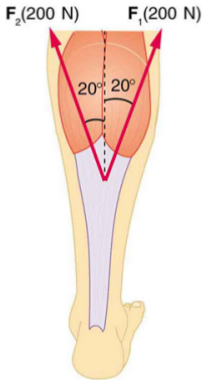
\includegraphics[width=0.175\textwidth]{figures/muscle.png}
\caption{\label{fig:muscle} The achilles tendon and the two muscles that connect to it.}
\end{figure}
\end{enumerate}

\section{Chapter 6: Further Applications of Newton's Laws, Friction and Drag}

\begin{enumerate}
\item A team of eight dogs pulls a sled with waxed wood runners on wet snow ($\mu_k = 0.1$). The loaded sled with its rider has a mass of 210 kg.  (a) Calculate the magnitude of the acceleration starting from rest if each dog exerts a net force per dog of 185 N backward on the snow. (b) What is the magnitude of the acceleration once the sled starts to move? (c) How long before the sled reaches 6 m/s? \\ \vspace{2.0cm}
\item Calculate the maximum deceleration of a car that is heading down a $6^{\circ}$ slope under the following road conditions. You may assume that the weight of the car is evenly distributed on all four tires and that the coefficient of static friction is involved (no slipping).  Calculate for a car: (a) On dry concrete ($\mu_s = 1.0$). (b) On wet concrete ($\mu_s = 0.7$). \\ \vspace{2.5cm}
\item \textbf{Drag Force}.  Suppose the force of drag on a bicyclist is 100 N, if the cross-sectional area is effectively 0.75 m$^2$. (a) What is the drag force if the area drops to 0.25 m$^2$? (b) Suppose $C = 1$, and $\rho = 1.2$ kg/m$^3$.  What is the speed of the bicyclist at the new drag force?  \\ \vspace{1cm}
\item Two tugboats push on a barge at different angles (see Fig. \ref{fig:boat}).  The first tugboat exerts a force of $2\times 10^5$ N in the x-direction, and the second tugboat exerts a force of $3 \times 10^5$ N in the y-direction. The mass of the barge is $5 \times 10^6$ kg, and its acceleration is observed to be $0.1$ m s$^{-2}$.  What is the drag force of the water on the barge resisting the motion? \\ \vspace{2cm}
\begin{figure}[ht]
\centering
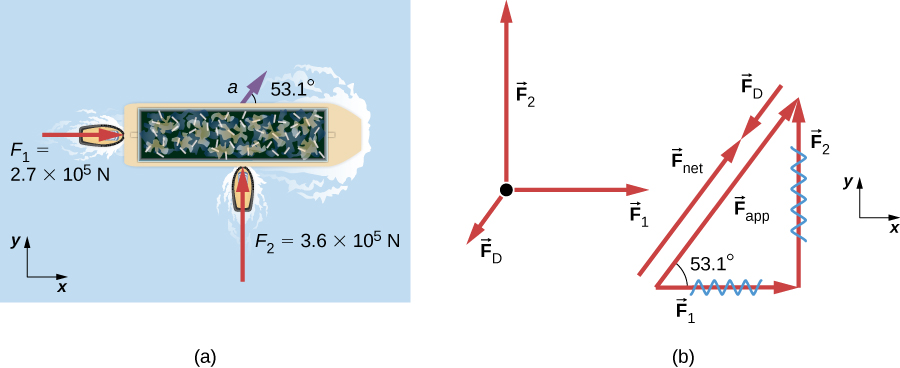
\includegraphics[width=0.6\textwidth]{figures/boat.jpeg}
\caption{\label{fig:boat}}
\end{figure}
\end{enumerate}

\section{Chapters 4, 5, and 6: Uniform Circular Motion and Gravitation}

\begin{enumerate}
\item In lacrosse, a ball is thrown from a net on the end of a stick by rotating the stick and forearm about the elbow. If the angular velocity of the ball about the elbow joint is 30.0 radians/second and the ball is 1.30 m from the elbow joint, what is the velocity
of the ball? \\ \vspace{1cm}
\item An ordinary workshop grindstone has a radius of 7.50 cm and rotates at 6500 rev/min.  Calculate the magnitude of the centripetal acceleration at its edge in m/s$^2$ and convert to g's. \\ \vspace{1cm}
\item What is the ideal banking angle for a gentle turn of 1.20 km radius on a highway with a 105 km/h speed limit, assuming everyone travels at the limit? \\ \vspace{1cm}
\end{enumerate}

\section{Chapter 8: Work and Kinetic Energy}

\begin{enumerate}
\item Suppose a 40 kg cart is pulled by a 100 N force that makes a 30 degree angle with the horizontal (see \ref{fig:cart}).  (a) Assumming no friction, what is the work done through a displacement of 10 meters? (b) Now assume that the frictional forces in Fig. \ref{fig:cart} are relevant.  There are \textit{four} wheels, and each wheel corresponds to $5$ N of frictional force.  What is the work done on the cart? (c) Including friction, if the cart starts from rest, what are the final kinetic energy and velocity of the cart? (d) What is the constant acceleration of the cart? (e) What is the power required to accelerate the cart? \\ \vspace{2cm}
\begin{figure}
\centering
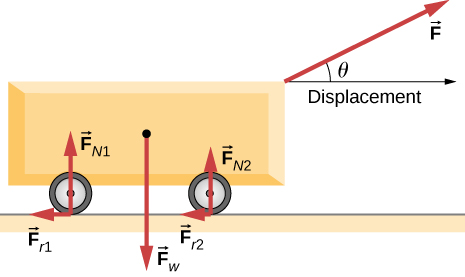
\includegraphics[width=0.35\textwidth]{figures/cart.jpeg}
\caption{\label{fig:cart} A cart is pulled by a force $\vec{F}$.  The weight, normal forces, and frictional forces are also shown.}
\end{figure}
\item Suppose electrical power costs \$0.2 dollars per kilo-Watt hour in your area.  Suppose your power consumption in your apartment is about 1000 Watts.  Estimate your monthly energy cost, that is, how much do you pay to run 1000 Watts for one month?
\end{enumerate}

\end{document}